%%%% fs-run-mapreduce Optimistic collision management
\label {fs-collision}

Deterministic execution is a desired property of any kind of system. If there are multiple possible outcomes, the developer needs to reason about which results are valid, which are equivalent and which are considered to be invalid.

To reduce outputs to only one possible result we impose two restrictions on our model: 

\begin{itemize}
  \item We require map function to be pure: return value is only determined by its input values, without observable side effects
  \item We impose a strict ordering requirements on the grouping's input
\end{itemize}

While the first requirement can be easily satisfied by moderating the provided business-logic, the second one is foreign to the distributed systems. Because of asynchrony and the possible existence of multiple paths between two nodes it is hard to deliver the right order. 

In this section we review common approaches for order enforcing, then we introduce our approach.

\subsection{Existing solutions}

There are two most common methods that are used to implement order-sensitive operators: in-order processing (IOP) \cite{Arasu:2006:CCQ:1146461.1146463, Cranor:2003:GSD:872757.872838, hammad2004optimizing} and out-of-order processing (OOP) \cite{Li:2008:OPN:1453856.1453890}.

According to IOP approach, each operation must enforce the total order on output elements that can be violated due to asynchronous nature of execution. Buffering is usually used to fulfill this requirement. For example, the implementation of the merge operator, in presence of a skew between input streams, must buffer the earlier one to enforce order on the output.

OOP is an approach that does not require order maintenance if it is not needed. In the case of ordering requirements, OOP buffers input items until a special condition is satisfied. This condition is supported by progress indicators such as punctuations \cite{Tucker:2003:EPS:776752.776780}, low watermarks \cite{Akidau:2013:MFS:2536222.2536229}, or heartbeats \cite{Srivastava:2004:FTM:1055558.1055596}. They go through the stream as ordinal items, but do not trigger business-logic of the operations. Each progress indicator carries meta-information and promises that there are no any elements with lesser meta-information. Therefore, indicators must be monotonic, but data items between two consecutive indicators can be arbitrarily reordered. Data sources periodically yield them.

While these methods are commonly adapted in practice we find them to have unpredictable latencies. In our system we employ an optimistic approach for handling out-of-order items.

\subsection{Optimistic approach}

As it was defined previously, only the grouping operation maintains a state and the state depends on the order of incoming items. Therefore, there is a need to enforce the right order to achieve deterministic processing.

As it was mentioned above, conservative methods for order enforcing can imply high latency overhead. Regarding our optimistic approach, we accept the fact that grouping can produce incorrect tuples. However, we guarantee that all correct tuples are eventually produced. The correctness of tuple means that this tuple would be generated if the order assumption was satisfied.

To eventually produce all correct tuples, we use an approach called {\it replay}. If an item arrives the grouping operation, according to the meta-information order, nothing is replayed and only the most recent window is produced. However, if an item is out-of-order, it is inserted in the bucket at the correct location, and all tuples, which contain this element, are reproduced. Thereby, replay guarantees that eventually all correct tuples are generated. At the same time, for tuples, that has been produced but became invalid, {\it tombstones} are sent.

Tombstones are ordinal data items but with a special flag in its meta-information. This flag means that tuples with such meta-information are invalid, and they should not leave the system. Tombstones have the same payloads as invalid items in order to go along the same path in the computational pipeline.

The example of replay is shown in Figure~\ref{grouping-replaying}, The green item is out-of-order. The output consists of the new valid items {\it (1, 2) and (2, 3)}, and the tombstone {\it (1, 3)} for the previously generated item.

\begin{figure}[htbp]
  \centering
  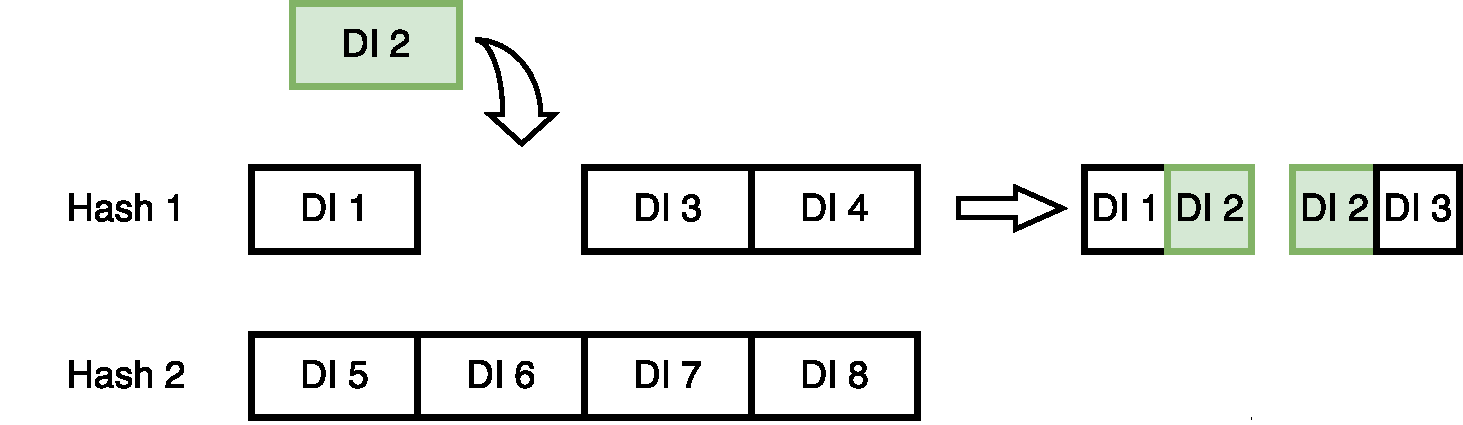
\includegraphics[width=0.48\textwidth]{pics/grouping-replaying}
  \caption{The replay in grouping with window = 2. The new items are generated on insertion}
  \label {grouping-replaying}
\end{figure}

In the case of the right order of input items, there are no redundant items produced.

The barrier filters out invalid elements, when corresponding tombstones arrive. It is partially flushed for some meta-information interval when there is a guarantee that there are no any out-of-order items and tombstones further up the stream for this range. The exact technique for providing such guarantee is defined in Section~\ref{fs-impl}.

\subsection{Advantages and limitations}

The proposed architecture's performance depends on how often reorderings are observed during the runtime. In the case when the order naturally preserved there is almost no overhead: when the watermark arrives, all computations are already done. The probability of reordering could be managed on a business-logic level and optimized by the developer. In experiments section it is shown that the computational nodes count is one of such parameters. Regarding the weaknesses, this method can generate additional items, which lead to extra network traffic and computations. Experiments, which are shown in the section~\ref{fs-experiments-section} demonstrate that the number of extra items is low.

